\section{Theoretische Grundlagen}
Stoffe haben die Möglichkeit unter bestimmten Bedingungen drei verschiedene Arten an Aggregatzuständen, also Phasen, anzunehmen.
Zu diesen zählen: fest, flüssig und gasförmig.
Maßgeblich für diese Bedingungen ist der Druck $p$ und die Temperatur $T$.  Zusammen bilden diese Variablen
ein pT-Diagramm. Dieses zeigt unter welchem Druck, mit welcher Temperatur,  welche Phase des Stoffes vorliegt.
Es existieren also in jeder Phase genau zwei Freiheitsgrade ohne das sich der Zustand des Stoffes verändert, eben bis dieser einen anderen Bezirk erreicht hat.
\begin{figure}
    \centering
    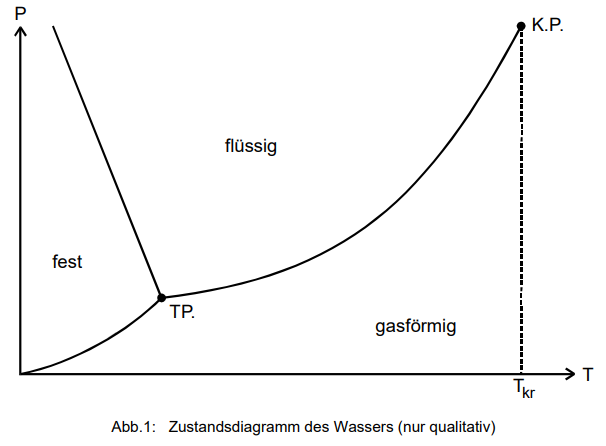
\includegraphics[width=\textwidth]{bilder/theoskizze1.png}
    \caption{Zustandsdiagramm des Wassers. \cite{skript}} 
    \label{fig:figtheo1}
\end{figure}
Die verschieden Aggregatzuständen werden durch Kurven getrennt, im Falle vom Wechsel: gasförmig $\longleftrightarrow$ flüssig,
nennt sich diese Begrenzung Dampfdurckkurve. (In der Darstellung \ref{fig:figtheo1}
die Kurve zwischen TP und KP)
Sollten Druck und Temperatur einen Zustand auf eben einer solchen Kurve erzeugen existiert der Stoff in beiden Phasen.
Um so zu bleiben reduzieren sich die Freiheitsgrade um einen Grad. Dieser Parameter wird Verdampfungswärme genannt und ist von der Temperatur
abhängig. 

\subsection{Mikroskopische Betrachtung bei Verdampfung und Kondensation}
Wenn im evakuiertem Raum die Flüssigkeit zum Verdampfen gebracht wird, lässt sich ein Druckanstieg feststellen.
Dieser resultiert aus der jetzt gasförmigen Flüssigkeit. Auf molekularer Ebene verlassen eben die Teilchen die Flüssigkeit, die genug kinetische Energie haben um sich von der Oberfläche zu entfernen. Dafür müssen sie mehr Kraft aufbringen können als die Molekularkraft des Stoffes zum Binden benötigt.
Diese zusätzliche Arbeit wird durch den Wärmevorrat des Stoffes unterstützt oder von außen hinzugefügt.
Als molare Verdampfungswärme $L$ versteht sich also das Maß an Energie, pro Mol der Flüssigkeit, um den Stoff bei gleicher Temperatur gasförmig zu machen.
Die Abgabe der aufgenommen Energie passiert durch Kondensation. Sie ist quasi das Gegenstück zur Verdampfung.
Kondensation führt der Flüssigkeit wieder Moleküle zurück, ebenso werden von der Oberfläche der Flüssigkeit wieder Teile des Gases aufgefangen.
Folglich, bei konstanten Bedingungen, verliert die Flüssigkeit eine Menge durch Phasenwechsel zu Gas, gewinnt aber auch eben gleichviel 
zurück durch Kondensation und Wiederaufnahme. Es hat sich ein Gleichgewicht mit konstantem Druck gebildet welcher Sättigungsdruck genannt wird.
Der Druck würde also bei zunehmender Temperatur, aufgrund der erhöhten kinetischen Energie und den folglich stärkeren Stößen, ansteigen.
Trotz Änderung des Volumens bleibt der Sättigungsdruck immer, nach entsprechender Anpassung durch Verdampfung oder Kondensation, gleich.

\subsection{Darstellung durch eine passende Differentialgleichung}
Die Natur des Systems lässt auf eine Lösung der Allgemeinen Gasgleichung vermuten,
\begin{equation}
    \label{eqn:gas}
    p \cdot V = R \cdot T
\end{equation}
welcher aber den Druck antiproportional zum Volumen wachsen lässt. Der Zusammenhang ist hier nicht zutreffend, da der Sättigungsdruck unabhängig vom Volumen ist.
\begin{figure}
    \centering
    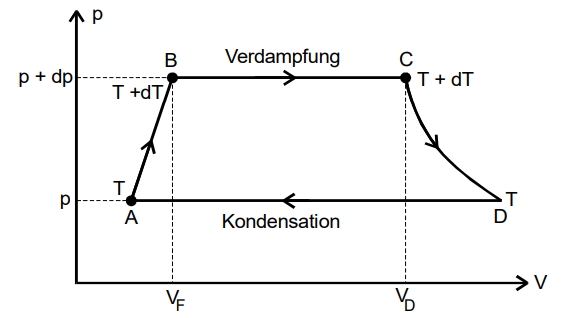
\includegraphics[width=\textwidth]{bilder/theoskizze2.png}
    \caption{Reversibler Kreisprozess. \cite{skript}} 
    \label{fig:figtheo2}
\end{figure}
Um also eine passende Darstellung für den Druck zu finden lässt sich zunächst ein anderer thermodynamischer Zusammenhang nutzen. 
Die Darstellung \ref{fig:figtheo2} zeigt die Änderung von Druck und Volumen einer Flüssigkeit mit Wärmekapazität $C_F$ in einem reversiblen Kreisprozess.
Beginnend bei Punkt A mit einem Druck $p$, einer Temperatur $T$ und einem Volumen $V_F$ ist das System ruhig und konstant. Die Temperatur wird so
gewählt, dass die einzige Phase in der sich die Flüssigkeit befinden kann flüssig ist.
Nach Zugabe der Energie $\Delta Q_{AB}$ in Form von Wärme steigt der Druck und mit ihr die Temperatur um jeweils $\Delta p$ bzw $\Delta T$.
Die Zugefügte Energie muss nach den Hauptsätzen der Thermodynamik im Stoff enthalten sein und es lässt sich sagen:
\begin{equation}
    \Delta Q_{AB} = C_F \cdot \Delta T
\end{equation}
Nach wiederholter Zugabe von Energie, hier als Verdampfungswärme um die Phase zu wechseln bei gleichem Druck, befindet sich das System im dritten Zustand
C. Hier ist die Flüssigkeit restlos verdampft und das Volumen hat sich vergrößert. Bei der Vergrößerung wurde eine Arbeit $A_{BC}$ verrichtet. 
Da sich das Volumen $V$ bei einem gewissen Druck $p +\Delta p$ um $\Delta V$ erweitert hat, lässt sich die Arbeit also beschreiben als.
\begin{equation}
\label{eqn:BC}
    -A_{BC} = (p+ \Delta p) \cdot (V_D-V_F)
\end{equation}
Hierbei wurde verwendet, dass $\Delta V$ eben der Abstand zwischen $V_F$ und $V_D$ ist. Die Arbeit wird vom Gas verrichtet um in eben diese Phase
zu kommen, folglich ist das Vorzeichen negativ. \\
Wird von hier das Gas auf die ursprüngliche Temperatur $T$ abgekühlt, wird wiederum Energie vom System abgegeben.
Die Tatsache, dass die Molwärme eines Stoffes multipliziert mit der Temperatur die Wärmeenergie angibt, führt auf den Zusammenhang.
\begin{equation}
    -\Delta Q_{CD} = C_D \cdot \Delta T
\end{equation}
$C_D$ beschreibt die Wärmekapazität des Gases und da die Wärme hier verschwindet ist auch das Vorzeichen negativ.
Die vierte Strecke findet bei konstanter Temperatur und konstantem Druck statt. Wie bei \eqref{eqn:BC} wird hier die Phase gewechselt, es wird also Wärmeenergie 
abgegeben.
\begin{equation}
    -A_{DA} = p \cdot (V_D - V_F)
\end{equation}
Summiert sich nun die hinzu - und abgegebene Wärme, muss diese nach dem ersten Hauptsatz der Thermodynamik gleich der summierten verrichteten Arbeit sein.
Also gilt:
\begin{align*}
     \Delta Q_{ges} &= C_F \cdot \Delta T - C_D \cdot \Delta T + L(T) + \Delta L - L(T) \\
     \intertext{Das $-L(T)$ entsteht durch die wieder abgezogene Verdampfungswärme bei der Kondensation}
    \Delta A_{ges} &= -((p+ \Delta p) \cdot (V_D-V_F)) \cdot -(p \cdot (V_D - V_F)) \\
    \hookrightarrow \Delta A_{ges} &= \Delta p (V_D - V_F) 
\end{align*}
Gleichsetzen liefert.
\begin{equation}
    \label{eqn:sum1}
    (C_F-C_D)\Delta T + \Delta L = (V_D - V_F) \Delta p
\end{equation}
Ebenso wird verlangt, dass nicht mehr Energie abgegeben wird als aufgenommen. Es lässt sich also nach dem zweiten Hauptsatz der Thermodynamik
sagen, dass die Summe aller reduzierten Wärmemengen null sein muss.
\begin{align}
\label{eqn:sum}
    \sum_i \frac{Q_i}{T_i} &= 0 \\
    \hookrightarrow \frac{C_F \cdot\Delta T}{T} + \frac{L + \Delta L}{T+ \Delta T}-\frac{C_D \cdot \Delta T}{T}-\frac{L}{T} &= 0
\end{align}
Mit der Temperatur $T$ multipliziert vereinfacht sich der Term. Außerdem wird genutzt, dass 
\begin{equation*}
    \frac{L+ \Delta L}{T + \Delta T} = \frac{L}{T} + \frac{\Delta L}{T} - \frac{L \Delta T}{T^2}
\end{equation*}
nach einer Reihenentwicklung bis zu erster Ordnung wie angegeben aussieht. Es folgt der Term.
\begin{equation}
    (C_F - C_D) \Delta T + \Delta L - \frac{L \Delta T}{T} = 0
\end{equation}
Der erste Teil ist bekannt und hat sowohl das als auch ein anderes Ergebnis. Aus \eqref{eqn:sum1} folgt der andere Zusammenhang.
\begin{equation}
    \label{eqn:dgl}
    (V_D-V_F) \Delta p = \frac{L \Delta T}{T}
\end{equation}  
Diese Differentialgleichung trägt den Namen Clausius-Clapeyronsche Gleichung und ist nur schwer lösbar aufgrund der vielfachen Abhängigkeiten von der 
Temperatur.

\subsection{Lösung der Differentialgleichung}
Um \eqref{eqn:dgl} vollständig zu lösen müssen vorerst Annahmen getroffen werden. 
Erstens soll gelten, dass das Anfgangsvolumen $V_F$ keine Auswirkung auf die Differenz $V_D - V_F$ haben soll. Zweitens wird eingeführt, dass 
sich das einzig relevante Volumen $V_D$ nach den Regeln der idealen Gasgleichung verhält \eqref{eqn:gas}. Drittens soll $L$ sowohl von der Temperatur
als auch vom Druck abhängig sein.
Es folgt die Gleichung.
\begin{align}
\label{eqn:wichtig}
    \frac{R}{p} \Delta p &= \frac{L}{T^2} \Delta T \\
    \intertext{Integration auf beiden Seiten nach entsprechender Variabel und unter Anwendung der $e$-Funktion liefert}
    \hookrightarrow p &= p_0 \cdot \text{exp} \left(-\frac{L}{R} \cdot \frac{1}{T}\right)
\end{align}
Grundlage der Formel ist die Boltzmann-Statistik welche eben die kinetische Energie beschreibt die hoch genug für einen Phasenwechsel ist. 
TEST TEST TEST.